
\newpage

\section{File inclusion}

De nombreux langages de programmation permettent d'inclure des portions de code contenues dans d'autres fichiers que celui en cours d'exécution. Le mécanisme mis à disposition permet de recopier dans le script principal le code contenu dans un autre fichier. Cette procédure est transparente à l'œil de l'utilisateur et peut-être très avantageuse pour le développeur d'un site internet.

\begin{figure}[!h]
\begin{center}

\label{inclusion}
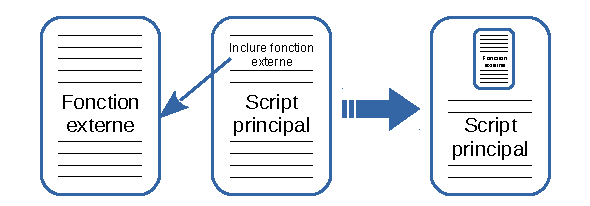
\includegraphics[scale=1.2]{images/include.pdf}

\caption{Mécanisme d'inclusion d'un fichier}

\end{center}
\end{figure}

En effet, inclure du code contenu dans un autre fichier permet, entre autre, les deux utilisations suivantes :
\begin{itemize}
\item inclure des portions de code différentes en fonction de choix de l'utilisateur ou de l'environnement de ce dernier;
\item inclure des portions de code utilisées dans plusieurs scripts (par exemple une fonction de connexion à une base de données) afin de ne pas avoir à recopier les mêmes lignes à différents endroits et de ne modifier qu'un seul fichier en cas de modification de la fonction.
\end{itemize}

Nous voyons donc que le premier point ci-dessus permet d'obtenir une réelle adaptabilité du code alors que le second point donne la possibilité au développeur d'écrire du code concis et factorisé. Nous allons cependant voir que ce mécanisme n'est pas dépourvu de vulnérabilités.


\subsection{Description de la vulnérabilité}

La principale vulnérabilité connue dans le mécanisme que nous venons d'expliciter intervient lorsque l'inclusion d'un script est géré par une variable pouvant être contrôlé par un attaquant. On se retrouve alors plutôt dans le premier cas d'utilisation indiqué, c'est à dire inclure des portions de code différentes en fonction de choix de l'utilisateur ou de l'environnement de ce dernier. En effet, dans le second cas d'utilisation, l'inclusion du fichier est généralement écrit "en dur" dans le script principal et ne peut donc pas être facilement modifié par un attaquant.

\begin{figure}[!h]
\begin{center}

\label{inclusion}
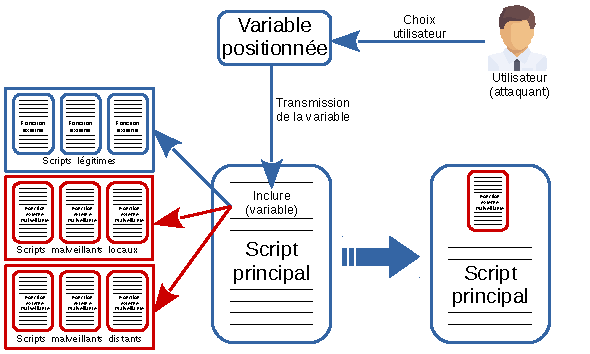
\includegraphics[scale=1.4]{images/include_hacked.pdf}

\caption{Vulnérabilité d'inclusion d'un fichier}

\end{center}
\end{figure}


ceci est un test

\subsection{Exploitation de la vulnérabilité}

\subsection{Contre-mesure}

\section{File upload}

\subsection{Description de la vulnérabilité}

\subsection{Exploitation de la vulnérabilité}

\subsection{Contre-mesure}

\section{Insecure CAPTCHA}

\subsection{Description de la vulnérabilité}

\subsection{Exploitation de la vulnérabilité}

\subsection{Contre-mesure}








